\section{The atomic limit}\label{sec:12.2}

A germanium atom that recoils with \SI{1}{keV} loses an electron to the continuum in one recoil in 580 according to the calculation of Ibe and collaborators, and in one recoil in 610 according to that of Cox and collaborators; in one recoil in 230 its electrons are left excited or ionized. Most of these events come from two shells, the $3d$ shell, bound by about \SI{30}{eV} and smaller than an angstrom, and the valence shell. A crystal of germanium keeps the first nearly as it is in the atom and rebuilds the second into bands. In the atom the Migdal entry \cref{eq:12.1-Skk} of the joint response can be evaluated to all orders in the momentum given to the electrons, and every number can be checked against a sum rule.

\subsection{The boost of a free atom}\label{sec:12.2-boost}

Take one atom at rest in its ground state, with a nucleus of mass $M$ at $\vect{X}$ and $N_e$ electrons at $\vect{r}_e$. Dark matter couples to the nucleus through $\ee^{\ii\vect{q}\cdot\vect{X}}$, to first order in the coupling. The Coulomb energy depends only on the positions of the electrons relative to the nucleus, $\vect{\rho}_e = \vect{r}_e - \vect{X}$. We trade $\vect{X}$ for the center of mass $\vect{R}_{\mathrm{cm}} = (M\vect{X} + m_e\sum_e\vect{r}_e)/m_A$ and keep the $\vect{\rho}_e$, with
\begin{equation}
  m_A = M + N_em_e ,
  \label{eq:12.2-mA}
\end{equation}
the mass of the atom up to the binding energy of its electrons, less than a part in $10^{6}$. The chain rule gives $\nabla_{\vect{X}} = (M/m_A)\nabla_{\vect{R}_{\mathrm{cm}}} - \sum_e\nabla_{\vect{\rho}_e}$ and $\nabla_{\vect{r}_e} = (m_e/m_A)\nabla_{\vect{R}_{\mathrm{cm}}} + \nabla_{\vect{\rho}_e}$. In the kinetic energy $-\nabla_{\vect{X}}^2/2M - \sum_e\nabla_{\vect{r}_e}^2/2m_e$ the cross terms between $\nabla_{\vect{R}_{\mathrm{cm}}}$ and $\nabla_{\vect{\rho}_e}$ cancel, and the terms in $\nabla_{\vect{R}_{\mathrm{cm}}}^2$ add up to $1/2m_A$. The Hamiltonian separates exactly,
\begin{equation}
  H = -\frac{\nabla_{\vect{R}_{\mathrm{cm}}}^2}{2m_A} + H_{\mathrm{rel}} , \qquad
  H_{\mathrm{rel}} = -\sum_e\frac{\nabla_{\vect{\rho}_e}^2}{2m_e} - \frac{1}{2M}\Bigl(\sum_e\nabla_{\vect{\rho}_e}\Bigr)^2 + V_{eN} + V_{ee} .
  \label{eq:12.2-Hint}
\end{equation}
The internal Hamiltonian is the clamped-nucleus Hamiltonian of \cref{sec:5.1} plus one term, the kinetic energy $(\sum_e\vect{p}_e)^2/2M$ of a nucleus that balances the momentum of its electrons. Its diagonal part turns $m_e$ into the reduced mass, and its off-diagonal part, $-M^{-1}\sum_{e<e'}\nabla_{\vect{\rho}_e}\cdot\nabla_{\vect{\rho}_{e'}}$, is the mass-polarization term of atomic physics. Both change energies and wavefunctions at relative order $m_e/M$.

The kick separates just as exactly. Since $\vect{X} = \vect{R}_{\mathrm{cm}} - (m_e/m_A)\sum_e\vect{\rho}_e$,
\begin{equation}
  \ee^{\ii\vect{q}\cdot\vect{X}} = \ee^{\ii\vect{q}\cdot\vect{R}_{\mathrm{cm}}}\;\exp\Bigl(-\ii\vect{q}_e\cdot\sum_e\vect{\rho}_e\Bigr) , \qquad
  \vect{q}_e = \frac{m_e}{m_A}\,\vect{q} = m_e\vect{v}_A ,
  \label{eq:12.2-cm}
\end{equation}
with $\vect{v}_A = \vect{q}/m_A$ the velocity of the recoiling atom. The first factor gives the whole atom the momentum $\vect{q}$ and the kinetic energy $q^2/2m_A$. The second acts on the internal state alone, as a momentum $-\vect{q}_e$ given to every electron. For hydrogen this is the separation of \cref{sec:6.1}. With $N_e$ electrons the center of mass still separates exactly; what the other electrons change is the internal Hamiltonian, through the mass-polarization term, and the boost mass, $m_A$ in place of the proton mass. The joint response \cref{eq:12.1-joint} of a gas of $\nd_T$ such atoms per unit volume, incoherent between atoms, is therefore
\begin{keyresult}[Migdal effect of a free atom]
\begin{gather}
  S_{\kappa\kappa}(\vect{q};\omega_l,\omega_e) = 2\pi\nd_T\,\delta\Bigl(\omega_l - \frac{q^2}{2m_A}\Bigr)\sum_fP_f(\vect{q})\,\delta(\omega_e - E_f + E_0) , \nonumber\\
  P_f(\vect{q}) = \Bigl|\Bigl\langle\Psi_f\Big|\exp\Bigl(-\ii\vect{q}_e\cdot\sum_e\vect{\rho}_e\Bigr)\Big|\Psi_0\Bigr\rangle\Bigr|^2 ,
  \label{eq:12.2-joint}
\end{gather}
with $\Psi_f$ and $E_f$ the eigenstates and energies of $H_{\mathrm{rel}}$ and $\vect{q}_e = m_e\vect{q}/m_A$. It holds to first order in the dark-matter coupling and to all orders in $q$, with no assumption about time.
\end{keyresult}
\noindent The term $f = 0$ is the line $\omega_e = 0$, the electron-following sector of \cref{eq:12.1-sectors}, with weight $P_0 = 1 - P_{\mathrm{Mig}}$. The rest is the Migdal entry. All of it sits on the line $\omega_l = q^2/2m_A$: a free atom has no phonons, and the lattice energy of every event is the recoil of the atom. \Cref{eq:12.2-joint} is the electron-cloud transition factor of Ibe and collaborators, who derive it in the same way and write the argument as the final velocity of the atom times $m_e$~\cite[Eqs.~(55), (57) and (73)]{ibe2018migdal}. Their phase $\ee^{-\ii\vect{q}_e\cdot\vect{x}}$ in the electron coordinates and the opposite sign of Kahlhoefer and Su~\cite[Eq.~(1)]{kahlhoefer2026probing} leave $|\cdot|^2$ unchanged.

\Cref{sec:6.1} reached the same structure from the other side, as the sudden boost \cref{eq:6.1-boost} with the velocity $v_N = q/M$ of the bare nucleus, and the leading entry \cref{eq:12.1-Skk} carries the same mass. Both are right to the order they claim. The exact separation fixes the next order: the boost mass is $m_A$, and at fixed $q$ the electrons receive $m_eq/m_A$, smaller than $m_eq/M$ by the factor $1 - N_em_e/m_A$. The electrons that follow the nucleus add their mass to it. This is the drag mass of \cref{eq:8.6-fsum-k}, $\delta M = N_em_e$ for an atom, and $M + \delta M = m_A$. The probability changes by $2N_em_e/m_A$, $5.5\times10^{-4}$ for silicon and $4.8\times10^{-4}$ for germanium, far below any other uncertainty of the calculation, but the counting of Migdal and lattice events in \cref{sec:12.5} needs it, and in a crystal the same role falls to $M_\kappa + \delta M_\kappa$ with the tensor drag mass of \cref{sec:8.6}. What the separation leaves to be solved is the internal problem. The states $\Psi_f$ are those of $H_{\mathrm{rel}}$, and the atomic calculations used below solve the clamped-nucleus problem instead, an error of relative order $m_e/M$ in each $P_f$.

The rate of a free-atom target follows from \cref{eq:8.2-spectrum} with the joint response \cref{eq:12.1-joint}. For a spin-independent coupling the nuclear vertex is $AF_N(q)$, the delta function of $\omega_l$ fixes $q = (2m_AE_R)^{1/2}$, and energy conservation needs $\omega_{\vect{q}} = E_R + \omega_e$. With the minimum velocity \cref{eq:1.3-vmin} at $\omega = E_R + \omega_e$, the free-recoil rate \cref{eq:11.4-LS} becomes
\begin{equation}
  \frac{\dd^2\mathcal{R}}{\dd E_R\,\dd\omega_e} = \frac{\rho_\chi\,\sigma_N}{2\mchi\,\mu_{\chi N}^2}\,F_N(q)^2\,\eta\Bigl(\frac{q}{2\mu_{\chi N}} + \frac{\omega_e}{q}\Bigr)\,\frac{\dd P}{\dd\omega_e}(q) ,
  \label{eq:12.2-rate}
\end{equation}
a rate per target atom, with $\mu_{\chi N}$ the reduced mass of the dark matter and the atom and $\dd P/\dd\omega_e = \sum_{f\neq0}P_f\,\delta(\omega_e - E_f + E_0)$. This is the rate of Ibe and collaborators~\cite[Eqs.~(91) and (92)]{ibe2018migdal}. The electronic energy raises $\vmin$ by $\omega_e/q$, and at fixed $\omega_e$ the recoil energy can no longer be arbitrarily small, since $\vmin$ grows without bound as $q \to 0$. The total deposit is at most the kinetic energy $\frac12\mchi v_{\mathrm{max}}^2$ of the dark matter, with the largest laboratory speed $v_{\mathrm{max}} = \SI{795}{km.s^{-1}}$ of the halo of \cref{sec:1.2}, \SI{35}{eV} at \SI{10}{MeV} and \SI{3.5}{keV} at \SI{1}{GeV}, and this, more than the probability, decides which shells a light particle can ionize.

\subsection{Shell probabilities at dipole order}\label{sec:12.2-dipole}

The electrons of an atom receive little momentum. A recoil energy $E_R$ gives them $q_e = m_e(2E_R/m_A)^{1/2}$, \SI{88}{eV} for germanium at $E_R = \SI{1}{keV}$, and the multipole parameter of \cref{sec:8.5} is $\xi_D = q_er_{\mathrm{orb}} = 0.07$ for its valence shell, of mean radius $2.9\,a_0$, and 0.02 for the $3d$ shell. The boost can be expanded. With $D_{\hat q} = \hat{\vect{q}}\cdot\sum_e\vect{\rho}_e$ the dipole operator of the electrons along the kick, the amplitude of an excited state is $-\ii q_e\langle\Psi_f|D_{\hat q}|\Psi_0\rangle$ plus terms of order $q_e^2$, and
\begin{equation}
  P_f = q_e^2\,\bigl|\langle\Psi_f|D_{\hat q}|\Psi_0\rangle\bigr|^2 , \qquad f \neq 0 ,
  \label{eq:12.2-dipole}
\end{equation}
at multipole order $n_D = 2$. Its corrections, of relative order $\xi_D^2$, come from the quadrupole and monopole terms of the boost and from the dipole term at second order. For hydrogen \cref{eq:12.2-dipole} sums to $q_e^2\langle z^2\rangle = q_e^2a_0^2$, the small-$v_N$ form of \cref{eq:6.1-P0}.

Two sums over final states are fixed without solving for any of them. Closure over $f \neq 0$ gives the total probability, and the double commutator of $D_{\hat q}$ with $H_{\mathrm{rel}}$ gives its first moment,
\begin{equation}
  P_{\mathrm{Mig}} = q_e^2\bigl(\langle D_{\hat q}^2\rangle - \langle D_{\hat q}\rangle^2\bigr) , \qquad
  \int\dd\omega_e\,\omega_e\,\frac{\dd P}{\dd\omega_e} = \frac{N_em_e}{M}\,E_R ,
  \label{eq:12.2-sums}
\end{equation}
with expectation values in the ground state. The total holds at dipole order; the first moment is exact to all orders in $q_e$. It is the f-sum rule \cref{eq:4.3-atomq} of the internal Hamiltonian, whose kinetic term \cref{eq:12.2-Hint} gives the double commutator $N_e/m_e + N_e^2/M = N_em_A/(m_eM)$, multiplied by $q_e^2/2$. At $E_R = \SI{1}{keV}$ it is \SI{0.27}{eV} for silicon, \SI{0.24}{eV} for germanium and \SI{0.23}{eV} for xenon: the mean energy the electrons take per recoil, carried by the small fraction of events that excite them. It is also the drag-mass term of \cref{eq:8.6-fsum-k}, $\vect{q}\cdot\delta M\cdot\vect{q}/2M^2$ with $\delta M = N_em_e$, up to a relative $m_e/M$. Any table of atomic Migdal probabilities must reproduce it, and the core shells, whose large excitation energies weight the sum, dominate it.

In practice the atom is described by one Slater determinant of orbitals, from a Hartree--Fock or Dirac--Hartree--Fock calculation, and \cref{eq:12.2-dipole} becomes a sum of one-electron transitions. The dipole operator is a sum of one-electron operators, so at this order it moves one electron, from an occupied orbital $a$ of a shell $n\ell$ to an empty orbital $b$. A transition into an occupied orbital is blocked by the Pauli principle. Summed over the orbitals of the shell and the degenerate final ones, the probability per unit energy of an ejected electron is
\begin{equation}
  \frac{\dd P_{n\ell}}{\dd E_{\mathrm{ej}}} = q_e^2\sum_{a\in n\ell}\sum_b\bigl|\langle b|\hat{\vect{q}}\cdot\vect{\rho}|a\rangle\bigr|^2\,\delta(E_{\mathrm{ej}} - \epsilon_b) ,
  \label{eq:12.2-shell}
\end{equation}
with $\epsilon_b$ the energy of a continuum orbital normalized per unit energy and $\omega_e = E_B + E_{\mathrm{ej}}$, with $E_B$ the binding energy of the shell. Bound empty orbitals $b$ give the excitation probabilities of the shell. Only $\ell' = \ell \pm 1$ is reached, and for a closed shell the result does not depend on the direction of $\vect{q}$. This is the leading-order formula of Ibe and collaborators~\cite[Eqs.~(86)--(90)]{ibe2018migdal}, and since every term carries $q_e^2$, a table at one $q_e$ gives every other. The orbitals are atomic Hartree--Fock orbitals and continuum states in the field of the ion, computed as for the ionization form factors of dark-matter--electron scattering (\cref{app:E.7}); \cref{eq:12.2-shell} is the dipole limit of the ionization form factor \cref{eq:2.2-fion}, with $q_e$ in place of $q$.

\begin{limitbox}[Atomic Migdal effect at dipole order][lim:12.2a]
For a free atom recoiling with $q$, each shell is ionized with $\dd P_{n\ell}/\dd E_{\mathrm{ej}} = q_e^2\sum_{a,b}|\langle b|\hat{\vect{q}}\cdot\vect{\rho}|a\rangle|^2\delta(E_{\mathrm{ej}} - \epsilon_b)$, $q_e = m_eq/m_A$, and the rate is \cref{eq:12.2-rate}~\cite[Eqs.~(73), (86)--(92)]{ibe2018migdal}.
\par\smallskip
{\centering
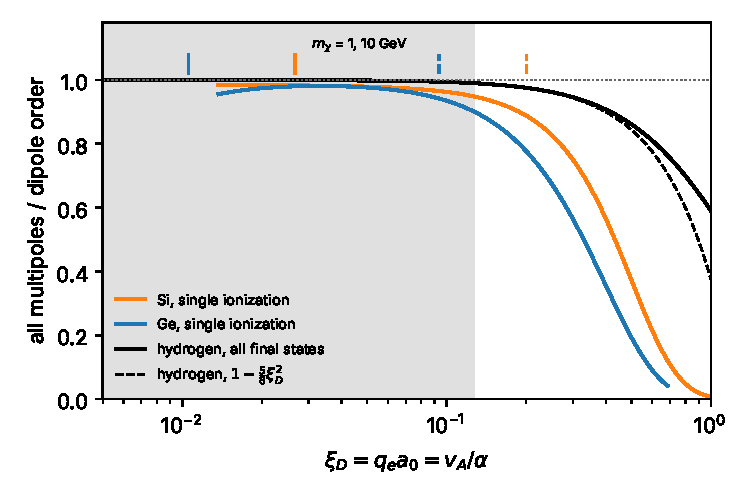
\includegraphics[width=\linewidth]{figures/ch12/limit12_2a.pdf}
\captionof{figure}{The Migdal probability with the full boost $\exp(-\ii\vect{q}_e\cdot\sum_e\vect{\rho}_e)$, all multipoles, divided by its dipole-order value, against $\xi_D = q_ea_0 = v_A/\alpha$. Black: hydrogen, all final states, $[1 - F_{1s}^2]/\xi_D^2$ from \cref{eq:6.1-P0}, exact. Dashed: its leading correction, $1 - \frac58\xi_D^2$. Orange and blue: single ionization of silicon and germanium atoms, Dirac--Hartree--Fock tables with multipoles up to $L = 10$ and at dipole order~\cite{cox2023precise}; a velocity-independent part of the tabulated full probabilities, $1.6\times10^{-4}$ (Si) and $1.3\times10^{-4}$ (Ge), which no transition between orthogonal states can have, is subtracted. Ticks: the largest recoil velocity for $\mchi = \SI{1}{GeV}$ (solid) and \SI{10}{GeV} (dashed), $v_A = 2\mu_{\chi N}v_{\mathrm{max}}/m_A$. Gray: $\xi_D \le 0.127$, where both atoms stay within \SI{10}{\percent} of the dipole result; silicon does so up to 0.188.}\label{fig:12-limit-2a}
\par}
\smallskip
Beyond $\xi_D \approx 0.13$ in germanium, reached by dark matter heavier than \SI{14}{GeV} (silicon: 0.19, \SI{9}{GeV}), an electron that is ionized can no longer leave the rest of the outer shell unexcited, and the single-ionization probability falls below the dipole value much earlier than in hydrogen.
\end{limitbox}

\noindent On the truncation label of \cref{eq:8.5-label} \cref{lim:12.2a} sits at $n_B = 2$, $n_D = 2$, $\mathfrak{M}$ = sudden and $\mathcal{K}$ = impulse. The dipole formula fails first in the outer shell, as Cox and collaborators showed. The exclusive probability of one ionization multiplies the transition of one electron by the probability that every other electron stays in its orbital. That product feels the bound--bound transitions of the outer shell at order $\xi_D^2$, with $r_{\mathrm{orb}}$ the outer-shell radius~\cite[Sect.~II\,C]{cox2023precise}. Below $\xi_D = 0.1$ all three curves of the box lie within \SI{7}{\percent} of one. The offset of about \SI{2}{\percent} of the two tabulated atoms at the smallest $\xi_D$, where the full and the dipole tables must agree, measures the numerical precision of the tables. For a particle of \SI{1}{GeV}, the endpoints are $\xi_D = 0.027$ in silicon and 0.011 in germanium, and \cref{eq:12.2-dipole} is as good as the atomic structure behind it.

\Cref{fig:12-atoms} shows the Migdal ionization spectra of silicon and germanium atoms at $E_R = \SI{1}{keV}$ against the electronic energy transfer $\omega_e$, the energy a detector records. The valence shells, bound by a few eV, dominate below a few tens of eV and fall as a power of $\omega_e$. The core shells open at their binding energies in $\omega_e$ and, because a tightly bound orbital couples to fast electrons, keep their spectrum flat up to energies of the order of their binding before they fall. The silicon $2p$ shell and the germanium $3d$ shell carry the spectrum from about \SI{50}{eV} to about a keV, and deeper shells beyond. Integrated over $\omega_e$, the ionization probability at \SI{1}{keV} is $2.09\times10^{-3}$ for silicon, of which the core shells $1s$, $2s$ and $2p$ give $7.9\times10^{-4}$, and $1.63\times10^{-3}$ for germanium in the Dirac--Hartree--Fock tables of Cox and collaborators. Xenon, from the tables of Ibe and collaborators, gives $1.98\times10^{-3}$. The three numbers are close because at fixed $E_R$ the factor $q_e^2 = 2m_e^2E_R/m_A$ falls with the mass of the atom while the dipole sum $\langle D_{\hat q}^2\rangle$ grows with the number of outer electrons. Two independent calculations exist for germanium, the relativistic local-potential one of Ibe and collaborators and the Dirac--Hartree--Fock one of Cox and collaborators. They agree within \SI{0.5}{\percent} on the $3d$ and $3p$ shells and within \SI{13}{\percent} on the valence $4p$ shell, and differ by \SI{6}{\percent} on the total, $1.73\times10^{-3}$ against $1.63\times10^{-3}$, the size of the uncertainty that the atomic structure adds.

\begin{figure}[tbp]
  \centering
  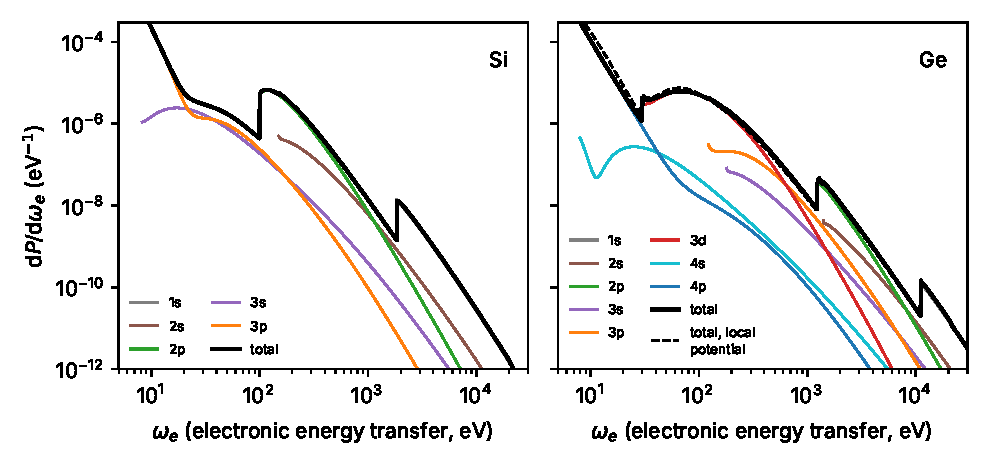
\includegraphics[width=\linewidth]{figures/ch12/fig12_2.pdf}
  \caption{Migdal ionization spectra of free silicon (left) and germanium (right) atoms at the recoil energy $E_R = \SI{1}{keV}$, per unit $\omega_e$ (electronic energy transfer), by initial shell (colors) and in total (black). Each shell is placed at $\omega_e = E_B + E_{\mathrm{ej}}$, its binding energy plus the kinetic energy of the ejected electron: measured binding energies of the core shells (\cref{sec:3.5}) and, for the valence shells, the measured first ionization energy of the atom, \SI{8.15}{eV} (Si) and \SI{7.90}{eV} (Ge), exact for the outer $p$ shell and a lower limit for the valence $s$ shell. Dipole-order Dirac--Hartree--Fock tables of Cox and collaborators~\cite{cox2023precise}, with the spin--orbit partners of each shell added, rescaled from $q_e = m_e\times10^{-3}$ to $q_e = m_e(2E_R/m_A)^{1/2}$, \SI{141}{eV} for silicon and \SI{88}{eV} for germanium. Dashed: total for germanium from the local-potential calculation of Ibe and collaborators~\cite{ibe2018migdal}, same rescaling. At other recoil energies every curve scales as $E_R$.}
  \label{fig:12-atoms}
\end{figure}

\begin{workedexample}{The Migdal probability of a germanium atom at \SI{1}{keV}}\label{we:12-germanium}
A germanium atom, $m_A = 72.630\,\mathrm{u} = \SI{67.654}{GeV}$, recoils with $E_R = \SI{1}{keV}$. Dark matter must be at least \SI{2.27}{GeV} to give it this energy at $v_{\mathrm{max}}$. The momentum transfer is $q = (2m_AE_R)^{1/2} = \SI{11.63}{MeV}$, the atom moves at $v_A = q/m_A = 1.72\times10^{-4}$, or \SI{51.5}{km.s^{-1}}, and each electron receives $q_e = m_ev_A = \SI{87.9}{eV}$, so that $q_ea_0 = v_A/\alpha = 0.024$. The tables of Ibe and collaborators are given at $q_e = m_e\times10^{-3} = \SI{511}{eV}$~\cite[Table~II]{ibe2018migdal}, and at dipole order we multiply them by $(87.9/511)^2 = 0.0296$.

The ionization probabilities are then $8.2\times10^{-4}$ from the $3d$ shell and $7.8\times10^{-4}$ from the $4p$ shell. The $3p$, $2p$ and $4s$ shells add $7.1\times10^{-5}$, $2.1\times10^{-5}$ and $1.8\times10^{-5}$, and the deeper shells less. The total is $1.73\times10^{-3}$: in this calculation one recoil in 580 ejects an electron. The shells with $n \le 3$ give $9.3\times10^{-4}$ of it. The table also lists transitions to bound orbitals. They add up to $8.75\times10^{-2}$ at the reference $q_e$, or $2.59\times10^{-3}$ at \SI{1}{keV}, more than the ionization, and the single transition $4s \to 4p$ gives $1.18\times10^{-3}$ of it. Every transition together has the probability $4.3\times10^{-3}$, one recoil in 230.

The sum rule \cref{eq:12.2-sums} checks the table. At the reference $q_e$ the exact first moment is $q_e^2N_e/2m_e = 32\times(\SI{511}{eV})^2/(2\times\SI{511}{keV}) = \SI{8.18}{eV}$. The ionization spectra, weighted with $\omega_e = E_B + E_{\mathrm{ej}}$ and the binding energies of the table, give \SI{7.28}{eV}, and the bound transitions, weighted with the differences of the tabulated level energies, \SI{0.63}{eV}. The tabulated transitions hold \SI{96.8}{\percent} of the moment; the rest lies in what the table omits, levels above $n' = 6$ and electrons faster than \SI{70}{keV}, and in the relativistic corrections to the nonrelativistic sum rule. At \SI{1}{keV} the moment is $(N_em_e/M)E_R = \SI{0.242}{eV}$, bound transitions included. Its ionization part, $\SI{7.28}{eV}\times0.0296 = \SI{0.215}{eV}$, carried by one event in 580, gives an ionizing event \SI{124}{eV} on average, and a $3d$ ionization \SI{135}{eV}.

Inside a germanium crystal the $3d$ shell keeps this probability. Its binding is \SI{29.4}{eV} below the valence maximum (\cref{sec:10.6}) where the table uses a computed \SI{35}{eV}, and the spectrum shifts with it. The valence part, $8.0\times10^{-4}$ of ionization and most of the bound transitions, does not carry over: in the crystal the $4s$ and $4p$ orbitals form the valence and conduction bands, $4s \to 4p$ is a transition across the gap, and \cref{sec:12.3} computes it from the loss function.
\end{workedexample}

\subsection{Core shells inside a crystal}\label{sec:12.2-cores}

\Cref{eq:12.2-joint} assumes three things that a crystal can violate: that the atom recoils freely, that it is isolated, and that the kick is over before the electrons respond.

\emph{Free recoil.} A nucleus bound in a lattice recoils like a free one once the recoil parameter $x_R = E_R/\langle\omega\rangle$ is large, above the impulse onset $x_R = 4$ of \cref{sec:11.4}: $q = \SI{92.5}{keV}$ and $E_R = \SI{164}{meV}$ in silicon, \SI{113}{keV} and \SI{95}{meV} in germanium. Above it the line $\omega_l = q^2/2m_A$ of \cref{eq:12.2-joint} becomes the impulse peak of \cref{eq:11.4-IA}, of relative width $x_R^{-1/2}$, $5\times10^{-3}$ at \SI{1}{keV} in germanium. The electronic factor is untouched. After the kick the neighbors pull the nucleus back on the time $1/\omega_{\mathrm{ph}}$, and the model of \cref{sec:6.1} found that this multiplies the excitation probability by $[1 - (\omega_{\mathrm{ph}}/\Delta E)^2]^{-2}$. For the germanium $3d$ shell, with the optical phonon of \SI{37.6}{meV} (\cref{tab:5-phonons}), the factor exceeds one by $3\times10^{-6}$, and for silicon $2p$ by $8\times10^{-7}$. Below the onset the lattice keeps the recoil in phonons, and the lattice factor is the multiphonon response of \cref{sec:12.4}.

\emph{Suddenness.} The kick lasts about as long as the dark matter takes to cross the nucleus, \SI{6e-21}{s} for germanium at $v_{\mathrm{max}}$ (\cref{sec:6.1}). Against the $3d$ excitation energy this is $\Delta E\,\tau_{\mathrm{acc}} = 3\times10^{-4}$, and for silicon $2p$ $7\times10^{-4}$, deep in the sudden region of \cref{fig:6-sudden}. The free atom needs no such condition, since \cref{eq:12.2-joint} is exact for it; in a crystal the condition is what lets the nucleus be treated as kicked first and decelerated afterward.

\emph{An isolated atom.} The electrons must move with their own nucleus and not with the crystal. A core orbital does. The silicon $2p$ shell has a mean radius of \SI{0.28}{\angstrom} and the germanium $3d$ shell \SI{0.39}{\angstrom}, against bonds of \SI{2.35}{\angstrom} and \SI{2.45}{\angstrom}. Their binding energies, \SI{99.5}{eV} (the spin--orbit centroid) and \SI{29.4}{eV} below the valence maximum, lie far below a valence band about \SI{12}{eV} wide. Such a shell forms a flat band whose orbitals are those of the atom, which first-principles calculations confirm for exactly these two shells (\cref{app:E.7}). The valence orbitals, of mean radius \SI{1.5}{\angstrom}, reach the neighbors, and their transitions become the band-to-band transitions of \cref{chap:10}. Their Migdal rate is the crystal formula of \cref{sec:12.3}, with the gap in place of the atomic binding. The atomic valence numbers above do not carry over: the crystal changes the valence channel by more than an order of magnitude (\cref{sec:12.3-atom}).

The mass that sets $q_e$ is $M_\kappa + \delta M_\kappa$, with the core electrons in $\delta M_\kappa$ exactly and the valence part a tensor (\cref{sec:8.6}), an effect of order $10^{-4}$. The largest correction is not in these three conditions but in the final state. Near its threshold the ejected core electron enters the conduction bands of the crystal and not the atomic continuum, and \cref{sec:10.6} found that the choice of final states changes the germanium $3d$ contribution to an electron-scattering rate by an order of magnitude near its opening. The atomic tables are reliable for core electrons ejected with tens of eV or more; within a few eV of the edge they are an estimate. With these provisos the core shells of a crystal take their Migdal probability from the atom, and \cref{sec:12.3} adds them to the valence rate.

\subsection{Excitation without ionization}\label{sec:12.2-excitation}

A kick can also leave an electron in an empty bound orbital. Kahlhoefer and Su proposed to detect this in superfluid helium, where an excited atom binds to a neighbor and the excimer emits an ultraviolet photon~\cite{kahlhoefer2026probing}. The first excited level of helium lies at \SI{20.6}{eV}, so a recoil far too weak to excite a neighbor by collision can still excite its own electrons. The probability is the sum of \cref{eq:12.2-joint} over the bound final states, and at dipole order, with the oscillator strengths \cref{eq:4.3-osc},
\begin{equation}
  P_{\mathrm{exc}} = q_e^2\sum_{f\,\mathrm{bound}}\bigl|\langle\Psi_f|D_{\hat q}|\Psi_0\rangle\bigr|^2 = \frac{q_e^2}{2m_e}\sum_{f\,\mathrm{bound}}\frac{f^{\mathrm{osc}}_{f0}}{E_f - E_0} .
  \label{eq:12.2-exc}
\end{equation}
The rate is \cref{eq:12.2-rate} with $\dd P/\dd\omega_e$ replaced by a sum of lines at the excitation energies, which is the form of Kahlhoefer and Su~\cite[Eq.~(6)]{kahlhoefer2026probing}. Only levels reached by the dipole operator appear: from the $1s^2$ ground state of helium, the $1snp\,{}^1P$ levels. With the measured oscillator strengths of these lines~\cite{kramida2024nist}, $0.276$ for $2\,{}^1P$ at \SI{21.22}{eV} and $0.073$ for $3\,{}^1P$ at \SI{23.09}{eV}, \cref{eq:12.2-exc} gives $P_{\mathrm{exc}} = 0.177\,(v_A/\alpha)^2$ for the first line, $0.220\,(v_A/\alpha)^2$ with the second, and $0.263\,(v_A/\alpha)^2$ with all lines up to the series limit at \SI{24.59}{eV}. A helium atom recoiling with \SI{10}{eV}, which dark matter of \SI{52}{MeV} can produce, has $v_A/\alpha = 0.010$ and is excited with probability $2.7\times10^{-5}$.

Any finite list of lines underestimates $P_{\mathrm{exc}}$, since every term of \cref{eq:12.2-exc} is positive; the first two helium lines hold \SI{84}{\percent} of it. A sharper statement compares the bound part with the ionization. Every bound level lies below the ionization energy $I$ and every continuum state above it. Weighting the oscillator strengths with $1/(E_f - E_0)$ therefore favors the bound part. Let $F_{\mathrm{exc}}$ and $F_{\mathrm{ion}}$ be the oscillator strength in the bound lines and in the continuum, and $P_{\mathrm{ion}} = P_{\mathrm{Mig}} - P_{\mathrm{exc}}$ the ionization probability. Then $P_{\mathrm{exc}} \ge q_e^2F_{\mathrm{exc}}/2m_eI$ and $P_{\mathrm{ion}} \le q_e^2F_{\mathrm{ion}}/2m_eI$, and
\begin{equation}
  \frac{P_{\mathrm{exc}}}{P_{\mathrm{ion}}} \ge \frac{F_{\mathrm{exc}}}{F_{\mathrm{ion}}} .
  \label{eq:12.2-bound}
\end{equation}
An estimate of the bound share from the oscillator strength alone, the share of the Thomas--Reiche--Kuhn sum \cref{eq:4.3-TRK} in the lines, is a lower bound. For hydrogen the lines hold 0.565 of the oscillator strength (\cref{sec:4.3}) but 0.717 of the dipole probability, of which the $2p$ level gives 0.555 and the levels with $n \le 3$ give 0.644.

\begin{limitbox}[Migdal excitation of bound final states][lim:12.2b]
A free atom recoiling with $q$ is left in the bound level $f$ with $P_f = |\langle\Psi_f|\exp(-\ii\vect{q}_e\cdot\sum_e\vect{\rho}_e)|\Psi_0\rangle|^2$, and the rate is the free-recoil rate times $\sum_fP_f\,\delta(\omega_e - E_f + E_0)$ over a list of levels~\cite[Eqs.~(1) and (6)]{kahlhoefer2026probing}; at dipole order this is \cref{eq:12.2-exc}.
\par\smallskip
{\centering
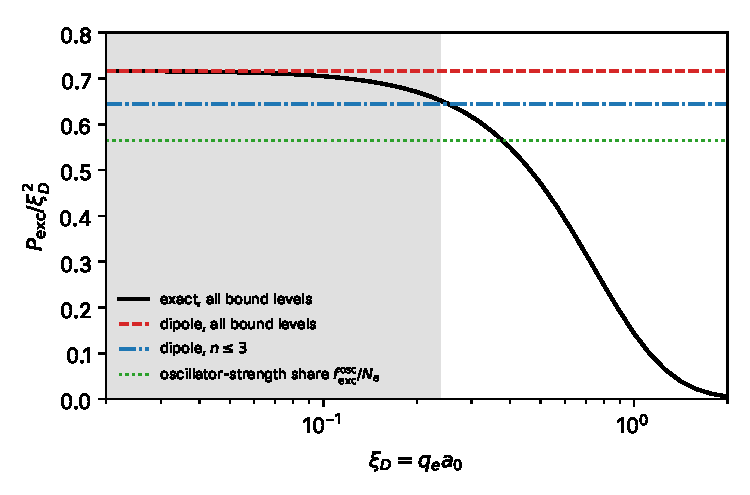
\includegraphics[width=\linewidth]{figures/ch12/limit12_2b.pdf}
\captionof{figure}{Probability that a kick leaves a hydrogen atom in a bound excited level, divided by $\xi_D^2 = (q_ea_0)^2$, against $\xi_D$. Solid: exact, the full boost and every bound level, from radial integrals with the spherical Bessel functions $j_\ell(q_er)$ for $n \le 40$ and $\ell \le 12$ and an $n^{-3}$ tail. Dashed: dipole order, all $np$ levels, 0.717. Dash-dotted: dipole order, levels with $n \le 3$ only, 0.644. Dotted: the bound share of the oscillator strength times the total dipole probability, 0.565, the lower bound \cref{eq:12.2-bound}. Gray: $\xi_D \le 0.24$, where the dipole sum over all levels is within \SI{10}{\percent} of the exact result.}\label{fig:12-limit-2b}
\par}
\smallskip
Beyond $\xi_D \approx 0.24$ the boost carries the electron more and more into the continuum, and the dipole sum overstates the bound probability, which falls to a fifth of it at $\xi_D = 1$.
\end{limitbox}

\noindent \Cref{lim:12.2b} sits at $n_B = 2$, $n_D = 2$, $\mathfrak{M}$ = sudden and $\mathcal{K}$ = impulse, as \cref{lim:12.2a} does. For dark matter lighter than \SI{1}{GeV} in helium, $\xi_D$ stays below 0.16, where the dipole sum for hydrogen is within \SI{4}{\percent} of the exact one; the finite list of lines, \SI{16}{\percent} short in helium, sets the larger error of the published estimate.

In germanium the bound transitions outnumber the ionizations. The table of \cref{we:12-germanium} lists $8.75\times10^{-2}$ in bound transitions against $5.86\times10^{-2}$ in ionization at the reference $q_e$, mostly $4s \to 4p$ and $4p \to 4d,\,5s$, and since the table stops at $n' = 6$ the true bound share is larger still. In a crystal these valence transitions do not exist as such. The bound final states of a crystal are excitons, whose lines below the pair continuum carry as much weight as the free pairs within $8E_x^b$ of the edge would (\cref{sec:10.5}). The Migdal entry \cref{eq:12.1-Skk} weights each final state with $\omega_e^{-4}$, which favors the lines below the edge for the same reason as \cref{eq:12.2-bound}. The exciton share of the Migdal spectrum is therefore at least the share of the lines in the electronic response near the edge. In silicon, with $E_x^b = \SI{14.7}{meV}$, and in germanium, whose indirect exciton is bound by about \SI{5}{meV}~\cite{macfarlane1957fine}, that share is negligible. In wide-gap crystals with binding energies of an eV and more it is not, and the lines are a separate, optically detectable signal (\cref{app:E.15}).
